%----------------------------%
% Contents slide

%----------------------------%


%----------------------------%
\begin{frame}
    \frametitle{Motivation}
    \small
\begin{columns}
\begin{column}{0.5\textwidth}
    Rolling element bearings are widely used in rotating machines. Their failure is one of the most frequent reasons for machine breakdown. 
    \\[1\baselineskip]
    This keynote will show the calculation of an elementary envelope spectrum to identify faults by monitoring for abnormalities in a bearing's
    \begin{itemize}
        \item Outer race
        \item Inner race 
        \item Fundamental train
        \item Rolling elements
    \end{itemize}
\end{column}
\begin{column}{0.5\textwidth}  %%<--- here
    \begin{figure}
        \centering
        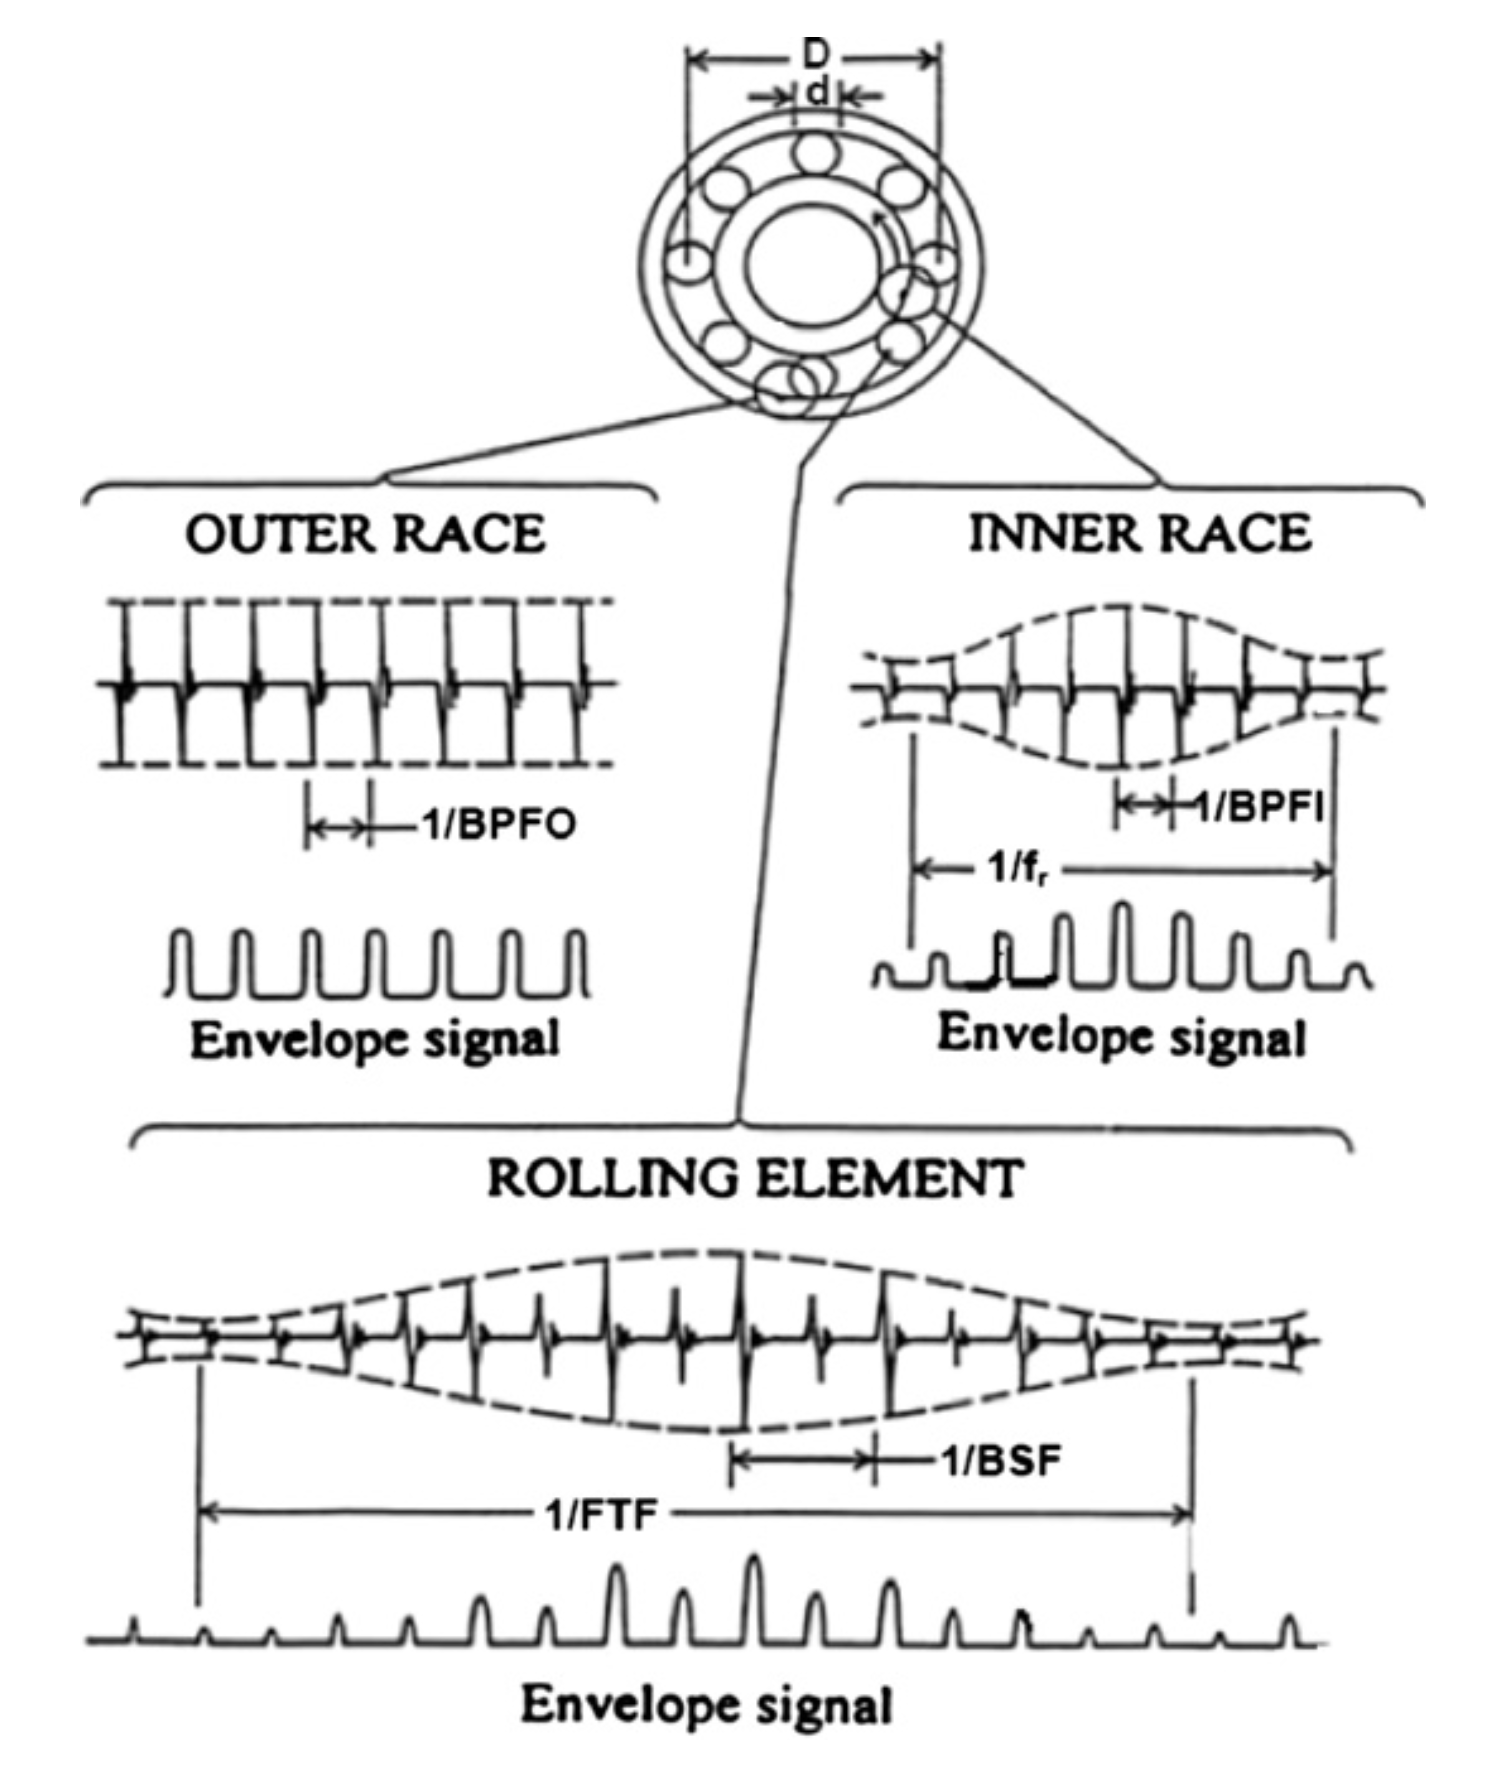
\includegraphics[width=\textwidth]{images/bearing.png}
        \caption{Typical signals and envelope signals from local faults in rolling element bearings. \cite{cm}.}
        \label{fig:spectrum}
    \end{figure}
\end{column}
\end{columns}
\end{frame}
